\documentclass{article}
\usepackage{geometry}
\usepackage{amsmath}
\usepackage{amssymb}
\usepackage{array}
\usepackage{tabularx}
\usepackage{setspace}
\usepackage{graphicx} % Required for including images
\usepackage{tikz}     % Required for watermarking
\usepackage{fancyhdr} % Required for custom headers/footers

\geometry{a4paper, margin=1in}
\setlength{\headheight}{33pt} % Fix header height for logo
\addtolength{\topmargin}{-21pt} % Adjust top margin accordingly

% --- Watermark setup ---
\usepackage{eso-pic}
\newcommand\BackgroundPicture{%
\put(\LenToUnit{0.5\paperwidth},\LenToUnit{0.5\paperheight}){%
\makebox(0,0)[c]{%
\tikz[opacity=0.08]\node{\includegraphics[width=1\paperwidth]{../oatutors_logo.png}};%
}%
}}
\AddToShipoutPicture{\BackgroundPicture}
% --- End Watermark setup ---

% --- Header setup for logo ---
\pagestyle{fancy}
\fancyhf{} % Clear all header and footer fields
\fancyhead[L]{\includegraphics[height=1.0cm]{../oatutors_logo.png}} % Logo on the left (slightly smaller for better proportion)
\fancyhead[C]{\textbf{11+ Non-Verbal Reasoning}} % Course title in center
\fancyhead[R]{\rightmark} % Section title on the right
\fancyfoot[C]{\thepage} % Page number in the footer
\renewcommand{\headrulewidth}{0.4pt} % Line under the header
\renewcommand{\footrulewidth}{0.4pt} % Line over the footer
% --- End Header setup ---


\begin{document}
\onehalfspacing

% This resets the page counter to 0 for the first page after the header setup
% \thispagestyle{fancy} % Apply fancy style to the first page too

\begin{center}
\textbf{\Large Shape Puzzles: Adding and Taking Away Patterns}
\vspace{0.2cm}
\end{center}

\hrule
\vspace{0.1cm}

\textbf{Topic:} Learning to Add and Subtract Shapes (Shape Math!) \\
\textbf{Target Age:} 10 years old \\
\textbf{Time:} 45 Minutes \\
\textbf{Resources:} Whiteboard/Projector, Fun Exercise Worksheets \\
\textbf{Website:} \texttt{https://oatutors.co.uk/}

\vspace{0.2cm}
\hrule
\vspace{0.3cm}

Get ready for an exciting adventure with shapes! Today we'll learn how to play with shapes like we do with numbers. We'll discover how to add shapes together and take them away from each other to solve fun puzzles!

\section{Let's Start Our Shape Adventure! (8 Minutes)}

\begin{tabularx}{\textwidth}{|>{\raggedright\arraybackslash}p{1cm}|>{\raggedright\arraybackslash}p{3cm}|>{\raggedright\arraybackslash}X|}
\hline
\textbf{Time} & \textbf{Activity} & \textbf{Description} \\
\hline
4 mins & Shape Math Magic! & Imagine shapes are like your toys! Just like you can add 2 apples + 3 apples = 5 apples, we can add shapes too! The magic rule is: Shape 1 + Shape 2 = Shape 3. Sometimes we also take shapes away: Shape 1 - Shape 2 = Shape 3. \\
\hline
4 mins & Fun Example Time! & Let's try together! Draw a box with a black circle + a box with a white square = a box with BOTH a black circle AND a white square! When we ``add'' shapes, we put them all together. When we ``take away,'' we remove the shapes that are the same. \\
\hline
\end{tabularx}

\section{Learning the Shape Rules! (12 Minutes)}

\begin{tabularx}{\textwidth}{|>{\raggedright\arraybackslash}p{1cm}|>{\raggedright\arraybackslash}p{3cm}|>{\raggedright\arraybackslash}X|}
\hline
\textbf{Time} & \textbf{Activity} & \textbf{Description} \\
\hline
8 mins & Two Super Cool Rules! & Let's learn the two amazing rules for shapes: \\
& & 1. \textbf{The 'Collecting' Rule ($X + Y = Z$):} When we collect shapes, we put ALL the shapes from the first two boxes into the third box. It's like putting all your toys in one big toy box! \\
& & 2. \textbf{The 'Disappearing' Rule ($X - Y = Z$ or $X \leftrightarrow Y = Z$):} This is like a magic trick! If the same shape appears in BOTH of the first two boxes, it disappears from the third box! Only shapes that appear in just ONE of the first boxes will stay. \\
\hline
4 mins & Let's Try Together! & Watch this magic trick with the Disappearing Rule: \\
& & \begin{tikzpicture}[scale=0.4] \\
& & \begin{scope}[xshift=0cm] \\
& & \fill[black] (0.2,0.2) circle (0.15); \\
& & \draw[thick] (0.5,0.1) rectangle (0.9,0.5); \\
& & \node at (0.5,-0.2) {\tiny F1}; \\
& & \end{scope} \\
& & \node at (1.1,0.3) {\tiny $\leftrightarrow$}; \\
& & \begin{scope}[xshift=1.3cm] \\
& & \draw[thick] (0.1,0.1) rectangle (0.5,0.5); \\
& & \fill[black] (0.6,0.2) -- (0.5,0.4) -- (0.7,0.4) -- cycle; \\
& & \node at (0.4,-0.2) {\tiny F2}; \\
& & \end{scope} \\
& & \node at (2.1,0.3) {\tiny =}; \\
& & \begin{scope}[xshift=2.3cm] \\
& & \fill[black] (0.1,0.2) circle (0.15); \\
& & \fill[black] (0.5,0.2) -- (0.4,0.4) -- (0.6,0.4) -- cycle; \\
& & \node at (0.4,-0.2) {\tiny F3}; \\
& & \end{scope} \\
& & \end{tikzpicture} \\
& & See how the White Square was in both boxes? It disappeared like magic! Let's say it out loud together: ``Same shapes in both boxes disappear!'' \\
\hline
\end{tabularx}

\section{Time to Practice Our Shape Magic! (15 Minutes)}

Let's try some fun puzzles together! For the disappearing trick puzzles, you can put your finger on shapes that appear in both boxes and watch them vanish!

\subsection*{Fun Shape Puzzles! (Worksheet)}
\textit{Instructions: Look at the first two boxes of shapes. Use our magic rules to find what should go in the third box. Remember: we either collect all the shapes together, or make the matching shapes disappear!}

\vspace{0.2cm}
\noindent\textbf{Puzzle 1: Collecting Shapes Together}

\begin{center}
\begin{tikzpicture}[scale=0.8]
    % Figure 1
    \draw[thick] (0,0) rectangle (1,1);
    \node at (0.5,-0.3) {Figure 1};
    
    % Plus sign
    \node at (1.5,0.5) {+};
    
    % Figure 2
    \fill (2.5,0.5) circle (0.15);
    \node at (2.5,-0.3) {Figure 2};
    
    % Equals sign
    \node at (3.5,0.5) {=};
    
    % Figure 3 (question mark)
    \draw[thick] (4,0) rectangle (5,1);
    \node at (4.5,0.5) {?};
    \node at (4.5,-0.3) {Figure 3};
\end{tikzpicture}
\end{center}

\textbf{Options:}
\begin{center}
\begin{tikzpicture}[scale=0.6]
    % Option A
    \draw[thick] (0,0) rectangle (1,1);
    \fill (0.8,0.8) circle (0.1);
    \node at (0.5,-0.4) {A};
    
    % Option B
    \draw[thick] (2,0) rectangle (3,1);
    \fill (2.5,0.5) circle (0.1);
    \node at (2.5,-0.4) {B};
    
    % Option C
    \fill[black] (4,0) rectangle (5,1);
    \fill[white] (4.5,0.5) circle (0.1);
    \node at (4.5,-0.4) {C};
    
    % Option D
    \draw[thick] (6,0) rectangle (7,1);
    \node at (6.5,-0.4) {D};
    
    % Option E
    \fill (8.5,0.5) circle (0.1);
    \node at (8.5,-0.4) {E};
\end{tikzpicture}
\end{center}



\vspace{0.2cm}
\noindent\textbf{Puzzle 2: The Disappearing Trick}

\begin{center}
\begin{tikzpicture}[scale=0.8]
    % Figure 1
    \begin{scope}[xshift=0cm]
        \fill[black] (0.5,0.7) -- (0.2,0.4) -- (0.2,0.1) -- (0.5,-0.2) -- (0.8,0.1) -- (0.8,0.4) -- cycle;
        \draw[white, thick] (0.2,0.6) -- (0.4,0.8) -- (0.6,0.6) -- (0.8,0.8) -- (0.6,1.0) -- (0.4,0.8) -- cycle;
        \fill[black] (0.8,0.8) circle (0.08);
        \node at (0.5,-0.5) {Figure 1};
    \end{scope}
    
    % Plus/Minus sign
    \node at (1.5,0.5) {$\leftrightarrow$};
    
    % Figure 2
    \begin{scope}[xshift=2cm]
        \fill[black] (0.5,0.7) -- (0.2,0.4) -- (0.2,0.1) -- (0.5,-0.2) -- (0.8,0.1) -- (0.8,0.4) -- cycle;
        \draw[white, thick] (0.3,0.3) -- (0.7,0.7);
        \draw[white, thick] (0.3,0.7) -- (0.7,0.3);
        \fill[black] (0.8,0.8) circle (0.08);
        \node at (0.5,-0.5) {Figure 2};
    \end{scope}
    
    % Equals sign
    \node at (3.5,0.5) {=};
    
    % Figure 3 (question mark)
    \draw[thick] (4,0) rectangle (5,1);
    \node at (4.5,0.5) {?};
    \node at (4.5,-0.5) {Figure 3};
\end{tikzpicture}
\end{center}

\textbf{Options:}
\begin{center}
\begin{tikzpicture}[scale=0.5]
    % Option A
    \begin{scope}[xshift=0cm]
        \draw[white, thick] (0.1,0.4) -- (0.3,0.6) -- (0.5,0.4) -- (0.7,0.6) -- (0.5,0.8) -- (0.3,0.6) -- cycle;
        \draw[white, thick] (0.2,0.2) -- (0.6,0.6);
        \draw[white, thick] (0.2,0.6) -- (0.6,0.2);
        \fill[black] (0.7,0.7) circle (0.06);
        \node at (0.4,-0.3) {A};
    \end{scope}
    
    % Option B
    \begin{scope}[xshift=2cm]
        \fill[black] (0.4,0.6) -- (0.2,0.4) -- (0.2,0.2) -- (0.4,0.0) -- (0.6,0.2) -- (0.6,0.4) -- cycle;
        \draw[white, thick] (0.2,0.2) -- (0.6,0.6);
        \draw[white, thick] (0.2,0.6) -- (0.6,0.2);
        \node at (0.4,-0.3) {B};
    \end{scope}
    
    % Option C
    \begin{scope}[xshift=4cm]
        \draw[white, thick] (0.1,0.4) -- (0.3,0.6) -- (0.5,0.4) -- (0.7,0.6) -- (0.5,0.8) -- (0.3,0.6) -- cycle;
        \draw[white, thick] (0.2,0.2) -- (0.6,0.6);
        \draw[white, thick] (0.2,0.6) -- (0.6,0.2);
        \node at (0.4,-0.3) {C};
    \end{scope}
    
    % Option D
    \begin{scope}[xshift=6cm]
        \fill[black] (0.4,0.4) circle (0.06);
        \node at (0.4,-0.3) {D};
    \end{scope}
    
    % Option E
    \begin{scope}[xshift=8cm]
        \fill[black] (0.4,0.6) -- (0.2,0.4) -- (0.2,0.2) -- (0.4,0.0) -- (0.6,0.2) -- (0.6,0.4) -- cycle;
        \draw[white, thick] (0.1,0.7) -- (0.3,0.9) -- (0.5,0.7) -- (0.7,0.9) -- (0.5,1.1) -- (0.3,0.9) -- cycle;
        \draw[white, thick] (0.2,0.2) -- (0.6,0.6);
        \draw[white, thick] (0.2,0.6) -- (0.6,0.2);
        \fill[black] (0.7,0.7) circle (0.06);
        \node at (0.4,-0.3) {E};
    \end{scope}
\end{tikzpicture}
\end{center}



\vspace{0.2cm}
\noindent\textbf{Puzzle 3: Tricky Disappearing Colors}

\begin{center}
\begin{tikzpicture}[scale=0.8]
    % Figure 1
    \begin{scope}[xshift=0cm]
        \draw[thick] (0,0) rectangle (1,1);
        \draw (0.5,0) -- (0.5,1);
        \draw (0,0.5) -- (1,0.5);
        \fill[gray] (0,0.5) rectangle (0.5,1); % Top-left shaded
        \fill[gray] (0.5,0) rectangle (1,0.5); % Bottom-right shaded
        \node at (0.5,-0.3) {Figure 1};
    \end{scope}
    
    % Minus sign
    \node at (1.5,0.5) {$-$};
    
    % Figure 2
    \begin{scope}[xshift=2cm]
        \draw[thick] (0,0) rectangle (1,1);
        \draw (0.5,0) -- (0.5,1);
        \draw (0,0.5) -- (1,0.5);
        \fill[gray] (0.5,0) rectangle (1,0.5); % Bottom-right shaded
        \fill[gray] (0,0) rectangle (0.5,0.5); % Bottom-left shaded
        \node at (0.5,-0.3) {Figure 2};
    \end{scope}
    
    % Equals sign
    \node at (3.5,0.5) {=};
    
    % Figure 3 (question mark)
    \draw[thick] (4,0) rectangle (5,1);
    \draw (4.5,0) -- (4.5,1);
    \draw (4,0.5) -- (5,0.5);
    \node at (4.5,0.5) {?};
    \node at (4.5,-0.3) {Figure 3};
\end{tikzpicture}
\end{center}

\textbf{Options:}
\begin{center}
\begin{tikzpicture}[scale=0.5]
    % Option A - All shaded
    \begin{scope}[xshift=0cm]
        \draw[thick] (0,0) rectangle (1,1);
        \draw (0.5,0) -- (0.5,1);
        \draw (0,0.5) -- (1,0.5);
        \fill[gray] (0,0) rectangle (1,1);
        \node at (0.5,-0.3) {A};
    \end{scope}
    
    % Option B - Top-left, top-right, bottom-left
    \begin{scope}[xshift=2cm]
        \draw[thick] (0,0) rectangle (1,1);
        \draw (0.5,0) -- (0.5,1);
        \draw (0,0.5) -- (1,0.5);
        \fill[gray] (0,0.5) rectangle (0.5,1); % Top-left
        \fill[gray] (0.5,0.5) rectangle (1,1); % Top-right
        \fill[gray] (0,0) rectangle (0.5,0.5); % Bottom-left
        \node at (0.5,-0.3) {B};
    \end{scope}
    
    % Option C - Top-left, bottom-right
    \begin{scope}[xshift=4cm]
        \draw[thick] (0,0) rectangle (1,1);
        \draw (0.5,0) -- (0.5,1);
        \draw (0,0.5) -- (1,0.5);
        \fill[gray] (0,0.5) rectangle (0.5,1); % Top-left
        \fill[gray] (0.5,0) rectangle (1,0.5); % Bottom-right
        \node at (0.5,-0.3) {C};
    \end{scope}
    
    % Option D - Top-left only
    \begin{scope}[xshift=6cm]
        \draw[thick] (0,0) rectangle (1,1);
        \draw (0.5,0) -- (0.5,1);
        \draw (0,0.5) -- (1,0.5);
        \fill[gray] (0,0.5) rectangle (0.5,1); % Top-left only
        \node at (0.5,-0.3) {D};
    \end{scope}
    
    % Option E - Bottom-left only
    \begin{scope}[xshift=8cm]
        \draw[thick] (0,0) rectangle (1,1);
        \draw (0.5,0) -- (0.5,1);
        \draw (0,0.5) -- (1,0.5);
        \fill[gray] (0,0) rectangle (0.5,0.5); % Bottom-left only
        \node at (0.5,-0.3) {E};
    \end{scope}
\end{tikzpicture}
\end{center}



\section{Let's Remember What We Learned! (10 Minutes)}

\begin{tabularx}{\textwidth}{|>{\raggedright\arraybackslash}p{1cm}|>{\raggedright\arraybackslash}p{3cm}|>{\raggedright\arraybackslash}X|}
\hline
\textbf{Time} & \textbf{Activity} & \textbf{Description} \\
\hline
4 mins & Quick Review Game & Let's remember our two super rules! Collecting shapes (putting them all together) and the disappearing trick (same shapes vanish). The disappearing trick is the most common magic in these puzzles! \\
\hline
6 mins & Take-Home Practice & Here are some fun puzzles to try at home! Remember to look carefully and decide: are we collecting shapes or making them disappear? \\
\hline
\end{tabularx}

\subsection*{Take-Home Fun Puzzles!}
\textit{Instructions: For each puzzle, decide if we're collecting shapes together or using the disappearing trick. Then find the missing shape!}

\vspace{0.2cm}
\noindent\textbf{Take-Home Puzzle 1: Find the Missing Shape in the Middle}

\begin{center}
\begin{tikzpicture}[scale=0.8]
    % Figure 1
    \begin{scope}[xshift=0cm]
        \draw[thick] (0,0) rectangle (1,1);
        \draw[thick] (0.5,0) -- (0.5,1); % Vertical line
        \node at (0.5,-0.3) {Figure 1};
    \end{scope}
    
    % Plus sign
    \node at (1.5,0.5) {$\leftrightarrow$};
    
    % Figure 2 (question mark)
    \draw[thick] (2,0) rectangle (3,1);
    \node at (2.5,0.5) {?};
    \node at (2.5,-0.3) {Figure 2};
    
    % Equals sign
    \node at (3.5,0.5) {=};
    
    % Figure 3
    \begin{scope}[xshift=4cm]
        \draw[thick] (0,0) rectangle (1,1);
        \draw[thick] (0,0.5) -- (1,0.5); % Horizontal line
        \node at (0.5,-0.3) {Figure 3};
    \end{scope}
\end{tikzpicture}
\end{center}

\textbf{Options for Figure 2:}
\begin{center}
\begin{tikzpicture}[scale=0.5]
    % Option A - Vertical line only
    \begin{scope}[xshift=0cm]
        \draw[thick] (0,0) rectangle (1,1);
        \draw[thick] (0.5,0) -- (0.5,1);
        \node at (0.5,-0.3) {A};
    \end{scope}
    
    % Option B - Both lines
    \begin{scope}[xshift=2cm]
        \draw[thick] (0,0) rectangle (1,1);
        \draw[thick] (0.5,0) -- (0.5,1);
        \draw[thick] (0,0.5) -- (1,0.5);
        \node at (0.5,-0.3) {B};
    \end{scope}
    
    % Option C - Horizontal line only
    \begin{scope}[xshift=4cm]
        \draw[thick] (0,0) rectangle (1,1);
        \draw[thick] (0,0.5) -- (1,0.5);
        \node at (0.5,-0.3) {C};
    \end{scope}
    
    % Option D - Empty square
    \begin{scope}[xshift=6cm]
        \draw[thick] (0,0) rectangle (1,1);
        \node at (0.5,-0.3) {D};
    \end{scope}
    
    % Option E - Diagonal line
    \begin{scope}[xshift=8cm]
        \draw[thick] (0,0) rectangle (1,1);
        \draw[thick] (0,0) -- (1,1);
        \node at (0.5,-0.3) {E};
    \end{scope}
\end{tikzpicture}
\end{center}



\vspace{0.2cm}
\noindent\textbf{Take-Home Puzzle 2: Collecting Shapes}

\begin{center}
\begin{tikzpicture}[scale=0.8]
    % Figure 1
    \begin{scope}[xshift=0cm]
        \draw[gray, thick] (0.4,0.5) -- (0.6,0.5); % Horizontal line of cross
        \draw[gray, thick] (0.5,0.4) -- (0.5,0.6); % Vertical line of cross
        \node at (0.5,-0.3) {Figure 1};
    \end{scope}
    
    % Plus sign
    \node at (1.5,0.5) {+};
    
    % Figure 2
    \begin{scope}[xshift=2cm]
        \draw[thick] (0,0) rectangle (1,1);
        \node at (0.5,-0.3) {Figure 2};
    \end{scope}
    
    % Equals sign
    \node at (3.5,0.5) {=};
    
    % Figure 3 (question mark)
    \draw[thick] (4,0) rectangle (5,1);
    \node at (4.5,0.5) {?};
    \node at (4.5,-0.3) {Figure 3};
\end{tikzpicture}
\end{center}

\textbf{Options:}
\begin{center}
\begin{tikzpicture}[scale=0.5]
    % Option A - Square with cross outside
    \begin{scope}[xshift=0cm]
        \draw[thick] (0.2,0.2) rectangle (0.8,0.8);
        \draw[gray, thick] (0.9,0.5) -- (1.1,0.5);
        \draw[gray, thick] (1.0,0.4) -- (1.0,0.6);
        \node at (0.5,-0.3) {A};
    \end{scope}
    
    % Option B - Square only
    \begin{scope}[xshift=2cm]
        \draw[thick] (0,0) rectangle (1,1);
        \node at (0.5,-0.3) {B};
    \end{scope}
    
    % Option C - Square with grey cross in center
    \begin{scope}[xshift=4cm]
        \draw[thick] (0,0) rectangle (1,1);
        \draw[gray, thick] (0.4,0.5) -- (0.6,0.5);
        \draw[gray, thick] (0.5,0.4) -- (0.5,0.6);
        \node at (0.5,-0.3) {C};
    \end{scope}
    
    % Option D - Square with black cross in center
    \begin{scope}[xshift=6cm]
        \draw[thick] (0,0) rectangle (1,1);
        \draw[black, thick] (0.4,0.5) -- (0.6,0.5);
        \draw[black, thick] (0.5,0.4) -- (0.5,0.6);
        \node at (0.5,-0.3) {D};
    \end{scope}
    
    % Option E - Grey cross only
    \begin{scope}[xshift=8cm]
        \draw[gray, thick] (0.4,0.5) -- (0.6,0.5);
        \draw[gray, thick] (0.5,0.4) -- (0.5,0.6);
        \node at (0.5,-0.3) {E};
    \end{scope}
\end{tikzpicture}
\end{center}

\newpage

\section*{Answer Key - For Teachers and Parents}

\subsection*{Worksheet Answers}

\textbf{Puzzle 1: Collecting Shapes Together}
\begin{itemize}
    \item \textbf{What's happening:} We're collecting shapes! The square from the first box and the circle from the second box both go into the third box.
    \item \textbf{Answer:} B - The box with both the square and the circle inside
\end{itemize}

\vspace{0.3cm}
\textbf{Puzzle 2: The Disappearing Trick}
\begin{itemize}
    \item \textbf{What's happening:} This is the disappearing trick! The black hexagon and black dot appear in BOTH boxes, so they disappear! Only the white star and white cross remain because they only appear in one box each.
    \item \textbf{Answer:} C - The box with just the white star and white cross
\end{itemize}

\vspace{0.3cm}
\textbf{Puzzle 3: Tricky Disappearing Colors}
\begin{itemize}
    \item \textbf{What's happening:} The gray color in the bottom-right appears in both boxes, so it disappears! Only the gray in the top-left stays because it's only in the first box.
    \item \textbf{Answer:} D - The box with gray only in the top-left corner
\end{itemize}

\subsection*{Take-Home Puzzle Answers}

\textbf{Take-Home Puzzle 1: Find the Missing Shape in the Middle}
\begin{itemize}
    \item \textbf{What's happening:} This is the disappearing trick working backwards! The first box has a vertical line. The third box has only a horizontal line. For the vertical line to disappear and leave just the horizontal line, the middle box must have BOTH lines (so the vertical cancels out).
    \item \textbf{Answer:} B - The box with both vertical and horizontal lines
\end{itemize}

\vspace{0.3cm}
\textbf{Take-Home Puzzle 2: Collecting Shapes}
\begin{itemize}
    \item \textbf{What's happening:} We're collecting shapes! The gray cross from the first box and the black square from the second box both go into the third box together.
    \item \textbf{Answer:} C - The black square with the gray cross inside it
\end{itemize}

\vspace{0.5cm}
\textit{Remember: When you see shapes being collected together, everything goes in the final box. When you see the disappearing trick, shapes that appear in both of the first boxes vanish, and only unique shapes remain!}

\end{document}